\documentclass[english,russian,a4paper,12pt]{article}
\usepackage[utf8]{inputenc}
\usepackage[T2A]{fontenc}
\usepackage{babel}
\usepackage{csquotes}

\usepackage{fullpage}
\usepackage{indentfirst}
\usepackage[font=small,labelfont=bf,labelsep=period]{caption}
\usepackage{graphicx}
\usepackage{wrapfig}
\usepackage{subcaption}
\usepackage{paralist}

\usepackage{amssymb, amsmath}

\usepackage{tikz}
\usetikzlibrary{arrows,fit,positioning,shapes.multipart}
\usetikzlibrary{shapes.geometric}

\usepackage[
	pdfauthor={Oleg Rogozin},
	pdftitle={Temperature ghost effect between two nonuniform heated parallel plates},
	colorlinks,pdftex, unicode]{hyperref}

\newcommand{\Kn}{\mathrm{Kn}}
\newcommand{\dd}{\:\mathrm{d}}
\newcommand{\pder}[2][]{\frac{\partial#1}{\partial#2}}
\newcommand{\pderder}[2][]{\frac{\partial^2 #1}{\partial #2^2}}

\usepackage[
	backend=biber,
	style=alphabetic,
	language=british,
	natbib=true,
	sorting=nyt,
	url=false,
	eprint=false,
	pagetracker,
	firstinits]{biblatex}
\bibliography{ghost_effect}

\title{Температурный эффект призрака между двумя неравномерно нагретыми параллельными пластинами}
\author{Рогозин Олег}
\date{}

\begin{document}

\maketitle
\tableofcontents

\section{Введение}

Для описания жидкости и газа в общем виде используются уравнения сохранения массы, импульса и энергии:
\begin{gather}
	\pder[\rho]{t} + \pder{x_i}(\rho v_i) = 0, \label{eq:mass}\\
	\pder{t}(\rho v_i) + \pder{x_j}(\rho v_i v_j + p_{ij}) = \rho F_i, \label{eq:momentum}\\
	\pder{t}\left[\rho\left(e+\frac{v_i^2}2\right)\right] +
		\pder{x_j}\left[\rho v_j\left(e+\frac{v_i^2}2\right)+v_i p_{ij}+q_j\right] = \rho v_j F_j. \label{eq:energy}
\end{gather}
Макроскопические параметры: \(\rho\) "--- плотность, \(v_i\) "--- скорость, \(p_{ij}\) "--- тензор напряжений,
\(e\) "--- удельная внутренняя энергия, \(q_i\) "--- тепловой поток. \(F_i\) "--- внешняя сила.
Для идеального одноатомного газа внутренняя энергия~\(e\) зависит только от температуры~\(T\):
\[ e = \frac32RT,\]
где \(R=k_B/m\) "--- удельная газовая постоянная. Давление выражается через уравнение состояния:
\[ p = \rho RT. \]

Для замыкания уравнений сохранения необходимо определить 
тензор напряжений \(p_{ij}\) и поток тепла \(q_i\).
Простейшие соотношения
\begin{equation}
	p_{ij} = p\delta_{ij}, \quad q_i = 0
\end{equation}
приводят~\eqref{eq:mass}--\eqref{eq:energy} к системе уравнений Эйлера,
описывающей поведение идеальной жидкости.

В общем случае в классической гидродинамике используется навье"--~стоксовкая система уравнений,
основанная на линейных законах Ньютона и Фурье:
\begin{gather}
	p_{ij} = p\delta_{ij} - \mu\left(\pder[v_i]{x_j}+\pder[v_j]{x_i}-\frac23\pder[v_k]{x_k}\delta_{ij}\right) -
		\mu_B\pder[v_k]{x_k}\delta_{ij}, \label{eq:stress_tensor}\\
	q_i = -\lambda\pder[T]{x_i}. \label{eq:heat_flow}
\end{gather}
Здесь \(\mu\) "--- вязкость, \(\mu_B\) "--- вторая вязкость, \(\lambda\) "--- теплопроводность.

Число Кнудсена \(\Kn\) определяет отношение длины свободного пробега
\begin{equation}\label{eq:ell}
	\ell = \frac{m}{\sqrt2\pi d_m^2 \rho}.
\end{equation}
к характерному размеру задачи \(L\):
\begin{equation}\label{eq:Knudsen}
	\Kn = \frac{\ell}L.
\end{equation}
Для модели твёрдых сфер радиус действия межмолекулярного потенциала взаимодействия \(d_m\)
совпадает с диаметром.

Для идеального газа вязкость \(\mu\) и теплопроводность \(\lambda\)
пропорциональны длине свободного пробега \(\ell\):
\[ \mu/\rho = f(T)(2RT)^{1/2}\ell, \quad \lambda/\rho = g(T)(2RT)^{1/2}R\ell. \]
Безразмерные функции \(f(T)\) и \(g(T)\) зависят от молекулярного потенциала.

Коэффициенты \(\mu\) и \(\lambda\) стремятся к нулю при \(\Kn\to0\).
Таким образом, в классической газовой динамике поле скоростей описывается уравнениями Эйлера везде,
кроме пограничного слоя и ударных волн.

Однако из системы уравнений Эйлера нельзя определить поле температуры.
Классическое уравнение теплопроводности получается из~\eqref{eq:energy} и~\eqref{eq:heat_flow}
в предположении отсутствия потоков газа \(v_i = 0\):
\begin{equation}\label{eq:heat_equation}
	\pder{x_i}\left(\sqrt{T}\pder[T]{x_i}\right) = 0.
\end{equation}
Здесь учтено, что теплопроводность идеального газа пропорциональна \(\sqrt{T}\).

При конечных значениях \(\Kn\) в уравнениях Навье"--~Стокса может возникать слабый конвекционный поток,
уравновешивающий член теплопроводности в~\eqref{eq:energy}.
Несмотря на своё исчезновение при \(\Kn\to0\), он конечным образом влияет на температурное поле.
Данная особенность асимптотического решения называется эффектом призрака~\cite{Sone2002, Sone2007}.
Оценить данное влияние можно только из кинетической теории.

\section{Асимптотический анализ уравнения Больцмана}
Подробный математический вывод приведённых ниже результатов~\cite{Bobylev1996} можно найти в~\cite{Sone2002}.

Стационарное уравнение Больцмана в отсутствие внешних сил в безразмерных переменных имеет вид:
\begin{equation}\label{eq:Boltzmann}
	\xi_i\pder[f]{x_i} = \frac1k J(f,f),
\end{equation}
\begin{equation}\label{eq:integral}
	J(f,g) = \frac12 \int(f'g'_*+g'f'_*-fg_*-gf_*)B\dd\Omega(\boldsymbol\alpha)\dd \boldsymbol\xi_*,
\end{equation}
где \(\Omega(\boldsymbol{\alpha})\) "--- телесный угол единичного вектора \(\boldsymbol\alpha\),
\(B\) "--- функционал межмолекулярного потенциала.
\[ k = \frac{\sqrt\pi}2\Kn.\]


Функция распределения \(f(x_i,\xi_i)\) раскладывается в ряд по \(k\)
\[ f = f_0 + f_1k + f_2k^2 + \cdots \]
следующим образом:
\begin{align*}
	J(f_0,f_0) &= 0, \\
	2J(f_0,f_m) &= \xi_i\pder[f_{m-1}]{x_i} - \sum\limits_{r=1}^{m-1}J(f_r,f_{m-r}), \quad m \in \mathbb{N}.
\end{align*}
Такое разложение впервые предложил Гильберт~\cite{Hilbert1912}. Далее будем использовать дополнительное условие
\begin{equation}\label{eq:Mach_constraint}
	\int\xi_if\dd\xi = O(k),
\end{equation}
означающее, что число Маха такого же порядка малости, что и число Кнудсена.

Макропараметры также разложим по числу Кнудсена:
\[ h = h_0 + h_1k + h_2k^2 + \cdots. \]

Конечным результатом анализа является следующая система уравнений для \(T_0\), \(v_{i1}\), \(p_2\)
на основе модели твёрдых сфер:
\begin{align}
	\pder{x_i}\left(\frac{p_0v_{i1}}{T_0}\right) &= 0, \label{eq:asymptotic1} \\
	\pder{x_j}\left(\frac{p_0v_{j1}v_{i1}}{T_0}\right) &= -\frac12\pder[p_2^\dag]{x_i} \notag\\
		&+ \frac{\gamma_1}2\pder{x_j}\left[\sqrt{T_0}\left(
			\pder[v_{i1}]{x_j}+\pder[v_{j1}]{x_i}-\frac23\pder[v_{k1}]{x_k}\delta_{ij}\right
		)\right] \notag\\
		&+ \frac{\gamma_7}{T_0}\pder[T_0]{x_i}\pder[T_0]{x_j}\left(
			\frac{v_{j1}}{\gamma_2\sqrt{T_0}} - \frac1{4p_0}\pder[T_0]{x_j}
		\right), \label{eq:asymptotic2} \\
	\pder{x_i}(p_0v_{i1}) &= \frac{\gamma_2}2\pder{x_i}\left(
		\sqrt{T_0}\pder[T_0]{x_i}
	\right). \label{eq:asymptotic3}
\end{align}
Давления \(p_0\), \(p_1\) являются константами,
\[ 
	p_2^\dag = p_2 + 
		\frac{2\gamma_3}{3p_0}\pder{x_k}\left(T_0\pder[T_0]{x_k}\right) -
		\frac{\gamma_7}{6p_0}\left(\pder[T_0]{x_k}\right)^2,
\]
Система \eqref{eq:asymptotic1}--\eqref{eq:asymptotic3} носит гидродинамический характер
и сравнима с уравнениями Навье"--~Стокса для сжимаемого газа (\(\rho_0 = p_0/T_0\)).
Формальная разница в дополнительных членах термических напряжений.
Кроме того, \(p_2^\dag\) не входит в уравнение состояния, поэтому определяется с точностью до константы.
Член \(\partial{p_2^\dag}/\partial{x_i}\) включён в систему,
как давление в уравнениях Навье"--~Стокса для несжимаемого газа,
что определяет соответствующие методы решения приведённой системы.

Для модели твёрдых сфер безразмерные коэффициенты переноса равны
\begin{alignat*}{2}
	\gamma_1 &= 1.270042427, &\quad \gamma_2 &= 1.922284066, \\
	\gamma_3 &= 1.947906335, &\quad \gamma_7 &= 1.758705.
\end{alignat*}

Первые два коэффициента соответствуют вязкости и теплопроводности:
\[ \mu = \frac{\sqrt\pi}2\gamma_1, \quad \lambda = \frac{5\sqrt\pi}2\gamma_2. \]

Граничные условия на границе с диффузным отражением имеют вид:
\begin{gather}
	T_0 = T_{w0}, \label{eq:bound:T} \\
	\left\{
	\begin{aligned}
		& \frac{(v_{j1}-v_{wj1})}{\sqrt{T_{w0}}}(\delta_{ij}-n_in_j) = 
			-\frac{K_1}{p_0}\pder[T_{w0}]{x_j}(\delta_{ij}-n_in_j), \\
		& v_{j1}n_j = 0.
	\end{aligned}
	\right. \label{eq:bound:v}
\end{gather}
Здесь \(n_i\) "--- нормаль к поверхности, \(v_{wj1}\), \(T_{w0}\) "--- скорость и температура границы.
\(K_1\) "--- безразмерный коэффициент температурного скачка. Для модели твёрдых сфер 
\[ K_1 = -0.6463. \]

\begin{wrapfigure}{r}{7cm}
	\vspace{-10pt}
	\centering
	\includegraphics{transport/Y1}
	\vspace{-15pt}
	\caption{Функция \(Y_1(\eta)\) кнудсеновского слоя для модели твёрдых сфер}\label{fig:Y1}
	\vspace{-5pt}
\end{wrapfigure}

Полученное решение не может точно удовлетворить кинетическому граничному условию ввиду
ввиду резкого изменения функции распределения у границы вдоль нормали к ней.
Поэтому необходимо вводить так называемую коррекцию кнудсеновского слоя:
\begin{equation}
	f = f_{FD} + f_K.
\end{equation}
Гидродинамическая часть \(f_{FD}\) представляет собой полученное ранее решение,
а \(f_K\) убывает экспоненциально от расстояния до границы \(\eta\):
\begin{equation}
	f_K = O\left(e^{-\eta}\right), \quad \eta = \frac{x_in_i}k.
\end{equation}

Ввиду малости числа Маха (\ref{eq:Mach_constraint}) \(f_K\) разлагается в ряд, начиная с первого порядка малости:
\[ f_K = f_{K1}k + f_{K2}k^2 + \cdots \]
Учёт кнудсеновского слоя вводит поправку для \(v_{i1}\) для модели твёрдых сфер:
\begin{equation}
	\left\{
	\begin{aligned}
		& \frac{v_{jK1}}{\sqrt{T_{w0}}}(\delta_{ij}-n_in_j) = 
			-\frac1{2p_0}\pder[T_{w0}]{x_j} Y_1\left(\frac\eta{T_{w0}}\right) (\delta_{ij}-n_in_j), \\
		& v_{jK1}n_j = 0.
	\end{aligned}
	\right. \label{eq:bound:v_K}
\end{equation}
Функция \(Y_1(\eta)\) табулирована, например, в~\cite{Sone2002, Sone2007} и изображена на рис.~\ref{fig:Y1}.

\subsection{Эффект призрака}

В системе \eqref{eq:asymptotic1}--\eqref{eq:asymptotic3} одновременно связаны величины 
из различных порядков разложения уравнения Больцмана по числу Кнудсена.
В гидродинамическом пределе (при \(\Kn\to0\)) член скорости первого порядка малости \(v_{i1}\)
вносит бесконечно малый вклад в поле скоростей \(v_i\),
однако конечным образом влияет на распределение температуры \(T=T_0\),
Другими словами, в континуальном мире у нас нет возможности измерить \(v_{i1}k\),
но тем не менее эта величина определяет поле температуры \(T\).
Этот эффект принято называть эффектом призрака~\cite{Sone2002, Sone2007}.

Видно, что при \(\Kn\to0\) газ в общем случае не описывается уравнением теплопроводности~\eqref{eq:heat_equation}.
Уравнение~\eqref{eq:asymptotic3} сходится к нему только в частном случае при \(v_{i1} = 0\).
Можно выделить три причины, по которым это условие не выполняется:
\begin{enumerate}
	\item Граница движется с инфинитезимальной скоростью: \(v_{wi} = v_{w1i}k\).
	\item Температура границы неравномерна (эффект теплового скольжения).
	\item Изотермические поверхности не параллельны (эффект термострессовой конвекции)~\cite{Kogan1976}:
		\begin{equation}
			e_{ijk}\pder[T_0]{x_j}\pder{x_k}\left(\pder[T_0]{x_l}\right)^2 = 0.
		\end{equation}
\end{enumerate}

\section{Постановка задачи}

Рассмотрим плоскую периодическую геометрию, как на рис.~\ref{fig:geometry}.
Газ расположен между двумя покоящимися (\(u_{wi} = 0\)) бесконечными параллельными пластинами,
разделёнными на единичное расстояние. Температура распределена на них по синусоидальному закону:
\begin{equation}
	T_w = 1-\alpha\cos(2\pi x).
\end{equation}
Будем рассматривать случай \(\alpha=1/2\).

\begin{wrapfigure}{r}{7.4cm}
	\vspace{-10pt}
	\centering
	\usetikzlibrary{decorations.pathreplacing}
	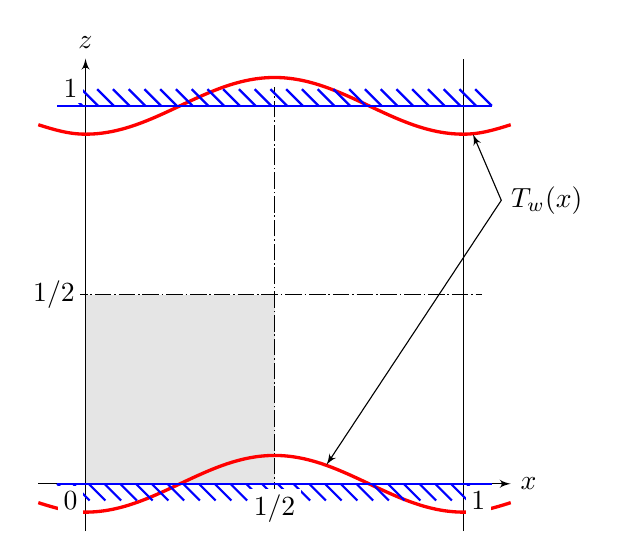
\begin{tikzpicture}[dashdot/.style={dash pattern=on .6pt off 1pt on 6pt off 1pt},
				interface/.style={postaction={draw, decorate, decoration=
					{border, angle=-45, amplitude=0.3cm, segment length=2mm}}},
				label/.style={fill=white, inner sep=2pt},
				>=latex', scale=1.2]
		\fill[gray!20] (0,0) -- (2,0) -- (2,2) -- (0,2) -- cycle;
		\draw[->] (-.5,0) -- (4.5,0) node[right] {\(x\)};
		\draw[->](0,-.5) -- (0,4.5) node[above] {\(z\)};
		\draw(4,-.5) -- (4,4.5);
		\draw[dashdot] (-.2,2) -- (4.2,2);
		\draw[dashdot] (2,-.2) -- (2,4.2);
		\draw[red, very thick] (-.5,-.2) sin (0,-.3) cos (1,0) sin (2,.3) cos (3,0) sin (4,-.3) cos (4.5,-.2);
		\draw[red, very thick] (-.5,3.8) sin  (0,3.7) cos (1,4) sin (2,4.3) cos (3,4) sin (4,3.7) cos (4.5,3.8);
		\draw[blue, thick, interface](-.3,0) -- (4.3,0);
		\draw[blue, thick, interface](4.3,4) -- (-0.3,4);
		\draw[<->] (4.1,3.7) -- (4.4,3) node[right] {\(T_w(x)\)} -- (2.55,.2);
		\node at (-.02,-.02) [below left, label] {0};
		\node at (4.02,-.02) [below right, label] {\(1\)};
		\node at (-.02,4.02) [above left, label] {\(1\)};
		\node at (-.05,2) [left, label] {\(1/2\)};
		\node at (2,-.05) [below, label] {\(1/2\)};
	\end{tikzpicture}
	\vspace{-15pt}
	\caption{Геометрия задачи}\label{fig:geometry}
	\vspace{-15pt}
\end{wrapfigure}

В силу симметрии задачи расчётная область представляет собой квадрат со стороной \(1/2\).
На рисунке выделена серым цветом.

Столкновения молекул газа описывается моделью твёрдых сфер. От пластин происходит полное диффузное отражение. 

Интерес представляет анализ сходимости при малых \(\Kn\) прямого численного моделирования уравнения Больцмана
к асимптотическому решению~\eqref{eq:asymptotic3} вместо классического уравнения теплопроводности~\eqref{eq:heat_equation}.
В~\cite{Bobylev1996} показана такая сходимость для модельного уравнения БКВ.

\section{Решение задачи в гидродинамическом пределе}

Для уравнения теплопроводности~\eqref{eq:heat_equation} граничные условия имеет простейший вид:
на твёрдой поверхности
\[ T = T_w, \]
на плоскостях симметрии
\[ \pder[T]{x_i}n_i = 0. \]
Получаемое таким образом температурное поле изображено на рис.~\ref{fig:isotemp:heat}.

\begin{figure}[ht]
	\centering
	\begin{subfigure}{0.45\textwidth}
		\centering
		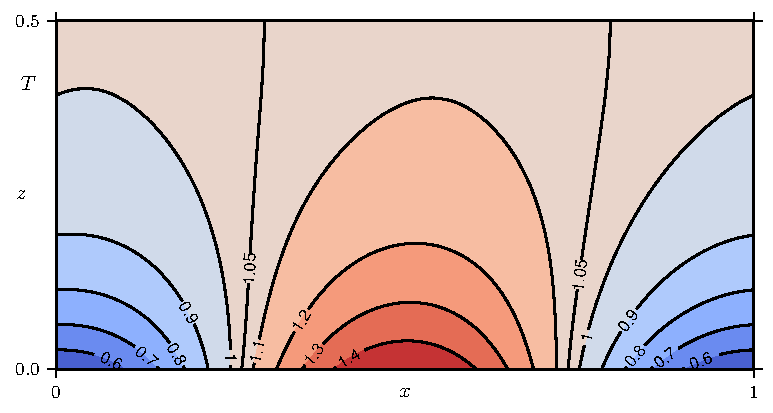
\includegraphics{fluid_dynamics/T_asym}
		\caption{асимптотическая теория}
		\label{fig:isotemp:asym}
	\end{subfigure}
	~
	\begin{subfigure}{0.45\textwidth}
		\centering
		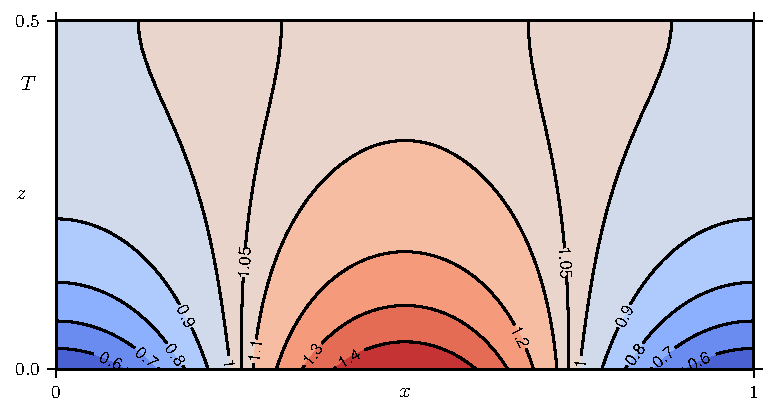
\includegraphics{fluid_dynamics/T_heat}
		\caption{уравнение теплопроводности}
		\label{fig:isotemp:heat}
	\end{subfigure}
	\caption{Изотермические линии в гидродинамическом пределе}\label{fig:isotemp}
\end{figure}

\begin{figure}[ht]
	\centering
	\begin{subfigure}{0.48\textwidth}
		\centering
		\includegraphics{fluid_dynamics/U_asym}
		\caption{\(u_{i1}\) при \(\Kn=0\)}\label{fig:velocity:asym}
	\end{subfigure}
	~
	\begin{subfigure}{0.48\textwidth}
		\centering
		\includegraphics{fluid_dynamics/U_kn001}
		\caption{\(u_{i1}\) при \(\Kn=0.01\) }\label{fig:velocity:asym_kn001}
	\end{subfigure}
	\caption{Стационарное поле скорости первого порядка (цветом показан её модуль)}\label{fig:velocity}
\end{figure}

Асимптотическое кинетическое решение~\eqref{eq:asymptotic1}"--~\eqref{eq:asymptotic3} выражается системой
\begin{align}
	\pder{x_i}\left(\frac{u_{i1}}T\right) &= 0, \label{eq:as:cont} \\
	\pder{x_j}\left(\frac{u_{i1}u_{j1}}{T}\right)
		&-\frac{\gamma_1}2\pder{x_j}\left[\sqrt{T}\left(
			\pder[u_{i1}]{x_j}+\pder[u_{j1}]{x_i}-\frac23\pder[u_{k1}]{x_k}\delta_{ij}\right
		)\right] \notag\\
		&- \frac{\gamma_7}T\pder[T]{x_i}\pder[T]{x_j}\left(\frac{u_{j1}}{\gamma_2\sqrt{T}} - \frac{1}4\pder[T]{x_j}\right) \notag\\
		&= -\frac1{2p_0}\pder[p_2^\dag]{x_i}, \label{eq:as:mom} \\
	\pder[u_{i1}]{x_i} &= \frac{\gamma_2}2\pder{x_i}\left(\sqrt{T}\pder[T]{x_i}\right). \label{eq:as:temp}
\end{align}
Здесь выполнена простая замена
\[ u_{i1} = p_0v_{i1}. \]
Индекс у температуры \(T\) исчез, поскольку при \(k=0\) получается точное равенство \[T=T_0.\]

Граничные условия на твёрдой поверхности получаются из~\eqref{eq:bound:T}"--~\eqref{eq:bound:v}:
\begin{align*}
	T &= T_w, \\
	u_{x1} &= -K_1\sqrt{T_w}\pder[T_w]{x}, \\
	u_{z1} &= 0.
\end{align*}

Ротор от~\eqref{eq:as:mom} позволяет исключить \(p_2^\dag\) из системы,
однако численное решение проще выполнить непосредственно в таком виде
общеизвестными итерационными методами для решения стационарных гидродинамических задач.
Уравнение непрерывности~\eqref{eq:as:cont} вместе с уравнением импульса~\eqref{eq:as:mom}
решаются, например, с помощью алгоритма SIMPLE~\cite{Caretto1972}.

В настоящей работе система уравнений~\eqref{eq:as:cont}"--~\eqref{eq:as:mom} решена
на готовой вычислительной платформе OpenFOAM\textregistered{}~\cite{Tabor1998}
с помощью специально разработанного солвера.

Искомое распределение температуры вычислено с большой точностью и показано
на рис.~\ref{fig:isotemp} в сравнении с решением уравнения теплопроводности.
На рис.~\ref{fig:velocity} изображено поле скоростей \(u_{i1}\) для предельного
и конечного чисел Кнудсена с учётом корректировки кнудсеновского слоя:
\[ u_{Kx1} = -\frac{\sqrt{T_w}}2\pder[T_w]{x} Y_1\left(\frac{z}{kT_w}\right), \quad u_{Kz1} = 0. \]

\section{Решение для произвольных чисел Кнудсена}

\begin{figure}[ht]
	\centering
	\begin{subfigure}[t]{0.48\textwidth}
		\centering
		\includegraphics{kinetic/T_kn001}
		\caption{поле температуры}\label{fig:kn001:T}
	\end{subfigure}
	~
	\begin{subfigure}[t]{0.48\textwidth}
		\centering
		\includegraphics{kinetic/U_kn001}
		\caption{поле скоростей}\label{fig:kn001:U}
	\end{subfigure}
	\caption{Прямое численное решение уравнения Больцмана для \(\Kn=0.01\)}\label{fig:kn001}
\end{figure}

Для решения задачи в произвольном диапазоне чисел Кнудсена будем использовать прямое решение
кинетического уравнения Больцмана методом конечных объёмов на основе
проекционного метода дискретных ординат~\cite{Tcheremissine1996}.

Используются пространственная и скоростная сетки объёмами
\[ V_{x_i} = 2500, \quad V_{\xi_i} = 11536 \]
соответственно.
Точность вычисления макропараметров составляет 0.1\%.

На рис.~\ref{fig:kn001} изображены поля температуры и скорости для случая \(\Kn=0.01\).

\section{Сравнение решений}

Чтобы наглядно изобразить сходимость численного метода прямого решения уравнения Больцмана,
рассмотрим зависимость температуры в заданных точках от числа Кнудсена (рис.~\ref{fig:temper}).

\newcommand{\tikzmarker}[2][]{\tikz[baseline=-0.5ex]\node[#1,draw,inner sep=#2] (0,0) {};}
\begin{figure}[ht]
	\centering
	\includegraphics{temper/temper}
	\caption{Значения температур в фиксированных точках: 
		\tikzmarker[fill=blue,circle]{2pt}, \tikzmarker[fill=green!50!black,circle]{2pt} --- прямое решение уравнения Больцмана;
		\tikzmarker[fill=blue,diamond]{2pt}, \tikzmarker[fill=green!50!black,diamond]{2pt} --- асимптотическое решение;
		\tikzmarker[fill=blue,square]{3pt}, \tikzmarker[fill=green!50!black,square]{3pt} --- уравнение теплопроводности.
	}\label{fig:temper}
\end{figure}

Видно, что достаточно гладко прямое решение сходится к асимптотическому.

\section{Заключение}

\begin{itemize}
	\item В гидродинамическом пределе (\(\Kn\to0\)) распределение газа является максвелловским,
	но макроскопические переменные в нём не удовлетворяют ни уравнениям Эйлера,
	ни уравнениям Навье"--~Стокса. Они определяются системой уравнений,
	содержащей члены более высокого порядка разреженности газа.
	\item Численный метод прямого решения уравнения Больцмана показывает сходимость
	с высокой точностью при моделировании слабо разреженного газа.
\end{itemize}



\printbibliography

\end{document}


